\documentclass[a4paper,11pt,twoside]{report}
\usepackage[T1]{fontenc}
\usepackage[frenchb]{babel} %active le mode français
\usepackage[latin1,utf8]{inputenc} % Mettre des accents
\usepackage[top=2cm , bottom=2cm , left=2cm , right=2cm]{geometry} %propriétés de notre page
\usepackage{amsmath} %liste de symboles et applications mathématiques
\usepackage{amsfonts} %idem
\usepackage{color} %Permet d'utiliser la couleur dans nos documents
\usepackage[usenames,dvipsnames]{xcolor}
\usepackage{listings} %Paquet de coloration syntaxique (langages)
\usepackage{hyperref} % Créer des liens et des signets 
\usepackage[babel=true]{csquotes} %permet les quotations (guillemets)
\usepackage{graphicx} %Importation d'image
\usepackage{fancyhdr} %en-tête et pieds de page+
\usepackage{lastpage} %permet d'obtenir le nombre total de page
\usepackage{multido}
%\usepackage{eurosym}
\usepackage{listingsutf8}
\usepackage{tikz}
\usepackage{ulem}
\usepackage{colortbl} %permet de mettre de personnaliser les colones des tabular
\usepackage{pdfpages}
\usepackage{appendix} %annexes
\setlength{\headheight}{15pt}
\lstset{language=C,
	breaklines=true,
	numbers=left,
	keywordstyle=\color{blue},
	commentstyle=\color{Gray},
	stringstyle=\color{red},
	tabsize=4,
	framexleftmargin=7mm,
	frame=single
	}
% Informations du rapport
\title {Rapport de TP \\ Problème de production de type ULS}
\author {Quentin Tonneau - Camille Drancourt}
\date{}
\renewcommand{\thesection}{\arabic{section}}
%Propriétés des liens
\hypersetup{
colorlinks=true, %colorise les liens  
urlcolor= blue, %couleur des hyperliens 
linkcolor= blue,%couleur des liens internes
citecolor=black
} 
%\setlength{\parindent}{0cm}
\addto\captionsfrench{
	\renewcommand{\chaptername}{Partie}
}

\fancypagestyle{plain}
{

	\fancyhead{}
	\fancyfoot{}
	\fancyfoot[LO RE]{\textit{Q.Tonneau - C.Drancourt}}
	\lhead{X7IO010}
	\rhead{Université de Nantes}
	\chead{Problème de production de type ULS}
	\fancyfoot[LE]{\thepage}
	\fancyfoot[RO]{\thepage}
}
\begin{document}
\thispagestyle{empty}
\Large{\uline{
\noindent Camille Drancourt}


\uline{Quentin Tonneau}}
\vfill
\begin{center}
\Huge{
 Rapport de Travaux Pratiques\\
 \textbf{Problème de Production de type ULS}}
 \vfill
 
\includegraphics[width=0.75\textwidth]{logo_univ_nantes.png}
 \vfill
\end{center}
X7IO010\hfill Novembre 2012
\newpage \pagestyle{empty}~
\tableofcontents
\newpage
\pagestyle{plain}
\chapter{Description du problème}
Le problème de planification de production étudié dans cet exercice est appelé \textit{Uncapacitated Lot-Sizing Problem}. Comme son nom l'indique, il n'y a dans ce cas précis aucune contrainte de capacité ou de limite de production.
Le plan de production est décomposé en T instances, dont on cherche à décider l'ouverture ou non ($y_t$), ainsi que la quantité d'éléments à produire $x_t$. L'ouverture d'une instance entraîne un coût fixe ($f_t$), ainsi qu'un coût unitaire de production ($p_t$).
Il faut impérativement subvenir aux demandes des clients pour tout instant $t$, mais il est possible à une instance $t$ de produire plus que nécessaire, et stocker l'ensemble de la ``surproduction'' ($s_t$) jusqu'à $t+1$ moyennant un coût unitaire de $h_t$.


Nous tentons dans cette analyse de résoudre quelques instances de ce problème via un algorithme de \textbf{branch \& bound}, et nous essayons de comprendre quelles sont les astuces de modélisation et les choix de résolution permettant d'améliorer au fur et à mesure notre rapidité de résolution.

\chapter{Le projet initial}
\section{La modélisation}
Les algorithmes de branch \& bound sont très utiles pour résoudre des problèmes en variables entières, en effectuant une série de résolution du problème ``relaché'' et en introduisant à chaque étape une nouvelle contrainte d'intégrité sur une des variables de décision.
Nous introduisons donc un modèle correspondant au problème ci-dessus, mais dont les variables entières ou binaires ($y_t$) ne possèdent pas de contraintes d’intégrité.

Voici le modèle proposé :
\[
 \left[ \begin{matrix}
         min z= & \displaystyle \sum_{t\in \{1...T\}} y_t \times f_t + x_t \times p_t + s_t \times h_t \\
         s/c & s_{t-1}+x_{t}& =d_t+s_t & \forall t\in \{0...T\} \\
         & y_t*M &\geq x_t \\
         &s_0&=0\\
         &s_t&=0\\
         &y_t,x_t,s_t&\geq 0
        \end{matrix}
 \right]
\]
La première contrainte, que nous appelons contrainte d'équilibre, impose l'absence de perte de produit lors de la production. En effet, l'ensemble des éléments entrants (stock précédent et production) doit être égal à l'ensemble des éléments sortants (ventes et stock).
La seconde contrainte implémente une constante M très grande imposant l'ouverture de l'instance si au moins un élément est produit par cette instance.
Les contraintes (3) et (4) indiquent l'état du stock au départ et à l'arrivé, fixés ici à 0.
\newpage
\section{L'algorithme}
Pour résoudre entièrement le problème, nous avons exécuté à la main l'algorithme du branch \& bound en effectuant les choix suivants :
\begin{itemize}
 \item Relâcher ou contraindre les variables $y_t$ à 0 ou 1.
 \item Toujours choisir la variable $y_t$ la plus proche de 0 et la fixer à 0 (dans un premier temps)
\end{itemize}

\section{L'implémentation}
Nous utilisons pour la résolution le solveur GLPK sous sa forme ``GNU Math Prog''. L'implémentation de la modélisation dans ce langage est donné en Annexe \ref{implementationlpsolve}.
Afin de contraindre une variable, nous ajoutons à chaque étape une ligne de type :
\begin{verbatim}
 s.t. contrX :y[A]=B;
\end{verbatim}
 avec A=$t$ et B$\in \{0,1\}$
 
 Nous fixons également M à 100, valeur arbitrairement grande.
\section{Résultats}
L'exécution de l'algorithme de branch\&bound nous permet d'obtenir l'arbre de la figure \ref{graph1}
\begin{figure}[h]
 \centering
 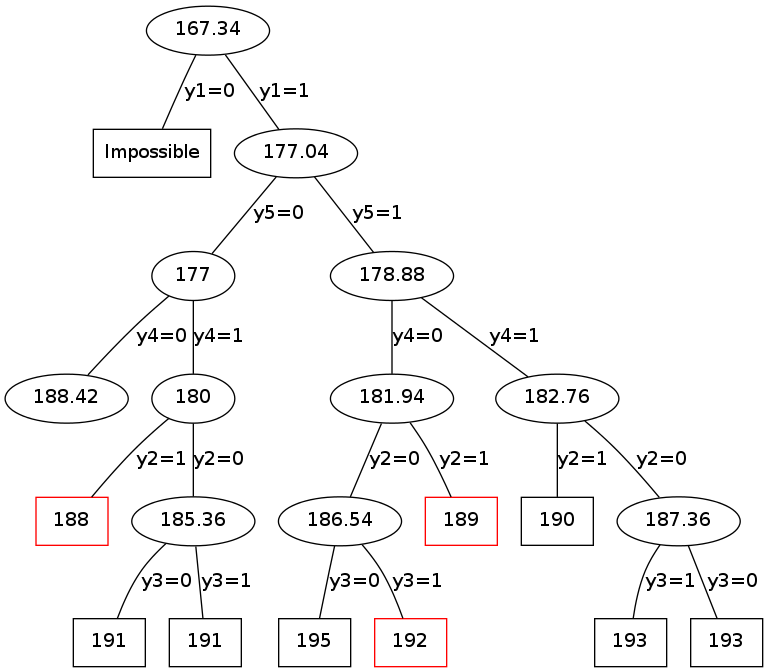
\includegraphics[width=0.8\textwidth]{graph1.png}
 \caption{Arbre initial}
 \label{graph1}
\end{figure}

On obtient un résultat optimal égal à 188, avec de très nombreuses branches et n\oe{}uds parcourus. Les choix de variables et de valeurs (algorithme de branch\&bound) ne sont pas optimaux, et il est sûrement possible d'améliorer notre modélisation ou notre système de résolution.
\chapter{Amélioration du modèle}
\section{Les valeurs des variables}
Le seul élément variable dans notre modélisation est $M$. En cherchant à améliorer la précision des résolution du problème relâché dans notre branch\&bound, nous arrivons à la conclusion suivante :

Plus M est petit, plus l'encadrement des valeurs possibles de chaque $y_t$ est petite. La valeur retournée par le solveur est donc plus proche de la valeurs maximum réelle.
Il faut cependant toujours conserver un M supérieur à la production maximale de chaque instance. On remarque, que la production maximale d'une instance est égale à la demande totale des clients. En effet, nous pourrions choisir de produire tous les éléments lors de la première instance, puis de répartir la production sur toutes les instances suivantes.
Dans l'instance donnée, $M$ doit être supérieure ou égale à 25. En modifiant M à 25, nous obtenons un arbre très similaire à la première résolution.

Afin d'améliorer encore notre modélisation, nous observons que la valeur maximale de M dépend de l'instance $t$. En effet, on ne peut produire au maximum que la demande totale \textbf{restante}.
Dans l'instance donnée, M devient donc un tableau de $5$ valeurs égales à $\{25, 22, 17, 11, 8\}$. Nous reprenons alors l'algorithme de branch\&bound, et nous obtenons l'arbre de la figure \ref{graph2}\\
\begin{figure}[h]
 \centering
 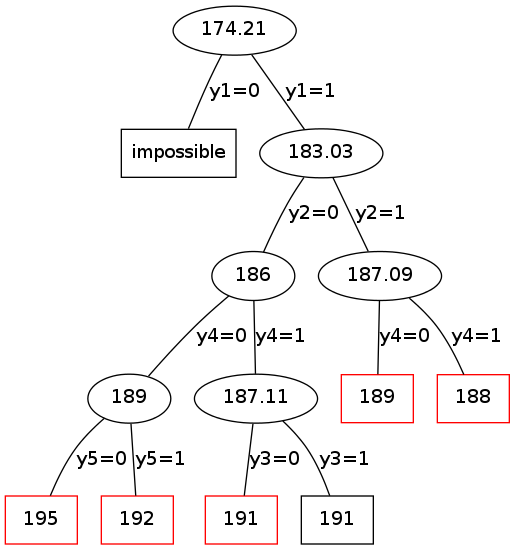
\includegraphics[width=\textwidth/2]{graph2.png}
 \caption{Modification de la valeur de M : tableau}
 \label{graph2}
\end{figure}



\section{Contraintes de coupes et inégalités valides}
Dans cette section, nous avons intégré à notre modèle une contrainte de type inégalité valide présenté par Laurence Wolsey. (\ref{equ1})
\begin{equation}
s_{t-1} <= d_{t}*(1-y_{t}) \label{equ1}
\end{equation}
L'inéquation (\ref{equ1}) exprime la volonté, pour une date $t$, de produire et de stocker à l'instance $t-1$ l'intégralité de la demande de la date $t$.
En effet, il est irrationnel dans un problème sans contrainte de capacité ($ULS$) de se limiter en quantité à l'instance la moins coûteuse.
Il est donc inutile d'ouvrir une instance dès que l'on a réussi à stocker suffisamment a l'instance précédente.
\begin{equation}
s_{t-1}+x_{t} = d_{t}+s_{t} \geq d_{t}
\end{equation}
\begin{center}\&\end{center}
\begin{equation}
y_{t}=0 \Rightarrow x_{t}=0
\end{equation}
Ainsi (\ref{equ1}) est toujours valide, et élague l'arborescence des solutions en forçant des variables $y_{t}$ relachées à se fixer à 0 .
Les résultats ont confirmé l'amélioration du modèle puisque l'arbre obtenue par Branch and Bound est réduit a deux feuilles (cf figure \ref{graph3}).
\begin{figure}[h]
 \centering
 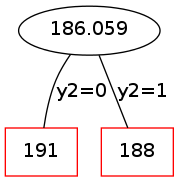
\includegraphics[width=\textwidth/4]{graph3.png}
 \caption{Avec Contrainte de Coupe}
 \label{graph3}
\end{figure}

\newpage
\section{Étude de la structure des solutions}
En observant la forme de la solution donnée, on peut effectuer la remarque suivante :



\textit{Si une instance est ouverte et précède une instance fermée, alors elle produit suffisamment pour $d_t$ et $d_{t+1}$.}




On peut alors voir la production à $t_i$ livrer directement $d_i$ et $d_{i+1}$, comme le montre la figure \ref{representation_graphique}. Le schéma fait disparaître la notion de stock et donne l'impression d'une livraison directe en revanche.


\begin{figure}[h]
 \centering
 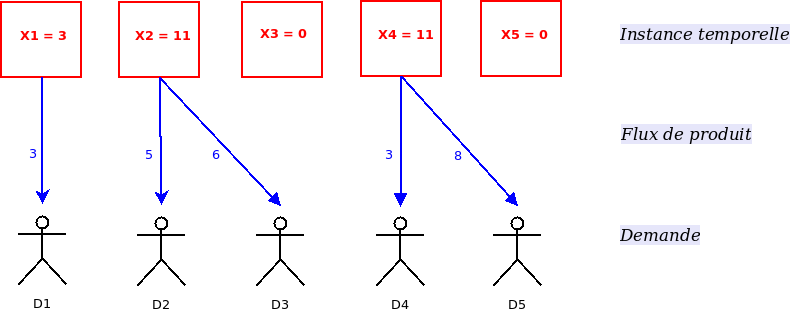
\includegraphics[width=\textwidth]{Diagramme1.png}
 \caption{Représentation visuelle de la solution}
 \label{representation_graphique}
\end{figure}
\section{Cas Wagner-Whitin}
Nous sommes dans un cas de coûts de Warner-Within lorsqu'il est systématiquement plus coûteux de produire et de stocker un produit pour une instance ultérieure, que de produire directement à l'instance $t$ (unitairement).
Un exemple de cas est donné dans le tableau \ref{warner1}
\begin{table}[h]
  \centering
 \begin{tabular}{|c|ccccc|}
\hline
$t$&1&2&3&4&5\\\hline\hline
$d_t$&3&5&6&3&8\\
$p_t$&3&4&4&8&3\\
$h_t$&2&1&5&1&-\\
$f_t$&10&8&6&4&2\\\hline
\end{tabular}
 \caption{Exemple de cas : Warner-Within}
 \label{warner1}
\end{table}

La logique nous amène alors à une résolution simple : On ne stocke jamais de produit, et on produit pour chaque instance $t$ la demande $d_t$ associée. Néanmoins, nous ne pouvons pas appliquer cette méthode directement.
En effet, cette solution est valable lorsque les coûts constants (activation d'une instance) sont très faibles ou tous (quasi) égaux. Si le gain total obtenu ($(p_t-(p_{t-1}+s_{t-1}))\times d_t$) est inférieur au coût initial de l'instance $t$ ($f_t$), alors il est plus intéressant de stocker que de produire (à $t$).
Le tableau ci-dessus (figure \ref{warner1}) en est un exemple : Avec une demande $d_2$ égale à 5, et un bénéfice unitaire $p_2-(p_1+s_1)$ de $1$, le gain total en produisant est de 5, alors que le coût initial de l'instance $t_2$ est de 8. Il est donc plus économique de produire en $t_1$ et de stocker (gain : 3).

\section{Modélisation finale}
Une troisième modélisation nous est proposé. On décompose ici la production de chaque instance, en sous-productions $w_{ij}$ (production de $i$ à destination de la demande $d_i$).
Ainsi modélisé, s'il y a une production $x_t>0$, alors $y_t$ sera forcément égal à 1, et le problème sera résolu en un appel au solveur. L'implémentation effectuée en Annexe \ref{pbfinal} nous donne en effet la valeur 188 (admissible) dès la racine de l'arbre.

\chapter{Conclusion}
En conclusion, la modélisation basique du problème ULS, est traité en des temps peu raisonnables par l'algorithme de Branch\&bound et calculé par un solveur comme le $GLPK$. Mais lorsque l'on complète le modèle avec des contraintes plus fines comme la contrainte de coupe ($3.1$), on obtient une solution dans des temps tres raisonnables.
Et si l'on arrive à identifier des cas particuliers comme celui de Wagner-Whitin la résolution devient triviale.
On voit au travers des essais et améliorations que l'algorithme de branch\&bound est efficace pour résoudre un problème en variables entières uniquement si la modélisation associée est efficace.
Les choix de parcours de l'arbre nous ne nous amènent pas rapidement à la meilleure solution, on peut donc imaginer qu'il existe des heuristiques/méta-heuristiques plus efficaces pour choisir les branches à explorer.
On peut par exemple prêter une attention particulière aux coûts duaux ainsi qu'à l'intervalle de stabilité des variables $y_t$.






\begin{appendices}
\chapter{Implémentation lpsolve}
\label{implementationlpsolve}
\begin{verbatim}
 #Données
param nbpostes;

set T:=1..nbpostes;
set T2:=0..nbpostes;
param M:=100;

param d{T};
param h{T};
param p{T};
param f{T};

#Variables de décision
var x{T} >=0;
var y{T} >=0;
var s{T2}>=0;

#Fonction objectif
minimize couts : sum{i in T} (y[i]*f[i] + x[i]*p[i] + h[i]*s[i]);

#Contraintes

s.t. Equilibre{i in T} : (s[i-1]+x[i])=(s[i]+d[i]);
s.t. Activation{i in T}: y[i]*M >= x[i];
s.t. contr1 :s[0]=0;
s.t. contr2 :s[nbpostes]=0;

#Résolution
solve;

#Affichange des res
display : s;
display : x;
display : y;
display : sum{i in T} (y[i]*f[i] + x[i]*p[i] + h[i]*s[i]);

data;

param nbpostes:= 5;
param d:= 1 3 2 5 3 6 4 3 5 8;
param p:= 1 2 2 4 3 6 4 8 5 10 ;
param h:= 1 3 2 2 3 3 4 2 5 0;
param f:= 1 10 2 8 3 6 4 4 5 2;

end;
\end{verbatim}

\chapter{Implémentation du problème final}
\label{pbfinal}
\begin{verbatim}
 #Variables de décision
var w11>=0;
var w12>=0;
var w13>=0;
var w14>=0;
var w15>=0;
var w21>=0;
var w22>=0;
var w23>=0;
var w24>=0;
var w25>=0;
var w31>=0;
var w32>=0;
var w33>=0;
var w34>=0;
var w35>=0;
var w41>=0;
var w42>=0;
var w43>=0;
var w44>=0;
var w45>=0;
var w51>=0;
var w52>=0;
var w53>=0;
var w54>=0;
var w55>=0;
var x1>=0;
var x2>=0;
var x3>=0;
var x4>=0;
var x5 >=0;
var y1>=0;
var y2>=0;
var y3>=0;
var y4>=0;
var y5>=0;
var s1>=0;
var s2>=0;
var s3>=0;
var s4>=0;

#Fonction objectif
minimize couts : 2*x1+4*x2+6*x3+8*x4+10*x5+3*s1+2*s2+3*s3
		 +2*s4+10*y1+8*y2+6*y3+4*y4+2*y5;


#Contraintes

s.t. contr1 : w11=3;
s.t. contr2 : w12+w22=5;
s.t. contr3 : w13+w23+w33=6;
s.t. contr4 : w14+w24+w34+w44=3;
s.t. contr5 : w15+w25+w35+w45+w55=8;

s.t. contr6 : w11<=3*y1;
s.t. contr7 : w12<=5*y1;
s.t. contr8 : w13<=6*y1;
s.t. contr9 : w14<=3*y1;
s.t. contr10 : w15<=8*y1;

s.t. contr11 : w22<=5*y2;
s.t. contr12 : w23<=6*y2;
s.t. contr13 : w24<=3*y2;
s.t. contr14 : w25<=8*y2;

s.t. contr15 : w33<=6*y3;
s.t. contr16 : w34<=3*y3;
s.t. contr17 : w35<=8*y3;

s.t. contr18 : w44<=3*y4;
s.t. contr19 : w45<=8*y4;

s.t. contr20 : w55<=8*y5;

s.t. contr21 : x1=w11+w12+w13+w14+w15;
s.t. contr22 : x2=w22+w23+w24+w25;
s.t. contr23 : x3=w33+w34+w35;
s.t. contr24 : x4=w44+w45;
s.t. contr25 : x5=w55;

s.t. contr26 : s1=x1-3;
s.t. contr27 : s2=x1+x2-8;
s.t. contr28 : s3=x1+x2+x3-14;
s.t. contr29 : s4=x1+x2+x3+x4-17;

#Résolution
solve;

#Affichange des res
display : y1;
display : y2;
display : y3;
display : y4;
display : y5;

display : x1;
display : x2;
display : x3;
display : x4;
display : x5;
display : 2*x1+4*x2+6*x3+8*x4+10*x5+3*s1+2*s2+3*s3
	  +2*s4+10*y1+8*y2+6*y3+4*y4+2*y5;
\end{verbatim}

\end{appendices}

\end{document}

